%%% Analyse for optimering af reguleringsloop %%%


\section{Gain-fase}
Reguleringssløjfen optimeres for, at opnå en større båndbredde. En større båndbredde vil give en hurtigere respons i systemet. Det vil betyde at systemet hurtige begynder at regulere ind ved ændringer på indgangen eller på loaden. Det resulterer i, at overshootet vil blive mindre.  

Der tages udgangspunkt i bode plottet for power modulet på figur~\ref{fig:MATLAB_power_module}. Ud fra kravene der er opstillet i afsnit~\ref{krav}, skal systemet minimum have en gain-margin på $10\decibel$ og en fase-margin på $50^\circ$. Ud fra figur~\ref{fig:MATLAB_power_module} ses det, at hvis der skal opnås en gain-margin på $10\decibel$, skal der tilføres en forstærkning på $8.5\decibel$. Ud fra bode plottet aflæses det, at ved, at løfte forstærkningen med $8.5\decibel$, vil der opnås en fase-margin på ca. $75^\circ$ og en båndbredde på ca. $4k\hertz$. 

\begin{figure}[H]
	\center
	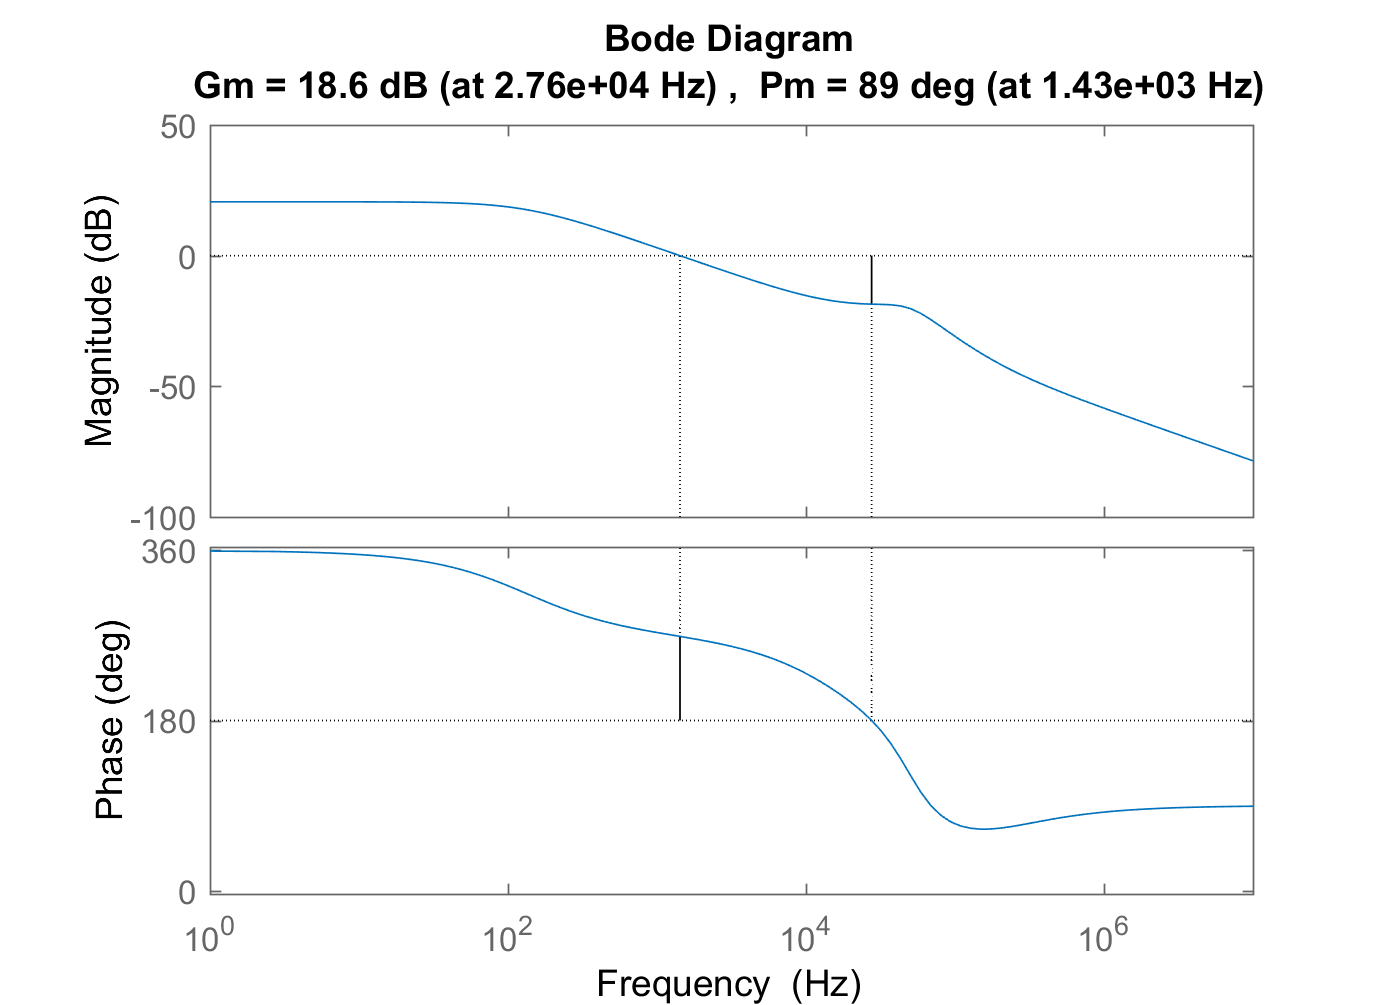
\includegraphics[max width=0.7\linewidth]{/tex/2iteration/billeder/MATLAB_power_module.PNG}
	\caption{Bode plot for power-modulet}
	\label{fig:MATLAB_power_module}
\end{figure}

\noindent Fremgangsmåden er den samme som ved 2. iteration. Feedback modstanden i fejlforstærkeren regnes ved at løse ligning~\ref{error_opamp_gain_3}.

\begin{equation} \label{error_opamp_gain_3}
g_{tot} = \frac{R_{comp}}{R_{par}} \cdot g_{FB}
\end{equation}

\noindent Hvor:
\newline \noindent $g_{tot}$ er den ønskede forstærkning i fejlforstærkeren. Der ønskes en forstærkning på $g_{totdb}8.5\decibel \Rightarrow g_{tot}=2.66gg$.
\newline \noindent $R_{comp}$ er feedbackmodstanden i fejlforstærkeren, som ønskes dimensioneret.
\newline \noindent $R_{par}$ er parallelmodstanden mellem $R_{FB1}$ og $R_{FB2}$. Den regnes til $R_{par}=2.244k\ohm$.
\newline \noindent $G_{FB}$ er forstærkningen i spændingsdeleren, og er tidligere regnet til $G_{FB}=0.12GG$.

\noindent De kendte værdier indsættes og ligningen løses for $R_{comp}$. Den fås til $R_{comp} = 49.8k\ohm$. Her rundes op til $49.9k\ohm$, som kan skaffes.

På figur~\ref{fig:MATLAB_total_2}, som er bodeplottet for det samlede system ved 2. iteration, ses det at fasen får et dyk, mellem ca. $80\hertz$ og ca. $400\hertz$. Det kommer fordi polen ved $132\hertz$ trækker fasen ned, mens det nulpunkt der er indsat ved $318\hertz$ trækker fasen op. Ved at flytte de punkter til samme frekvens, opnås en konstant fase ved lavere frekvenser. Derfor flyttes frekvensen for nulpunktet til $f_0=132\hertz$. Ud fra den nye modstand, og den nye knækfrekvens, regnes den nye kondensator. Det afrundes til $24.2nF$, da det kan skaffes.
\begin{equation} \label{c_comp_3}
c_{comp} = \frac{1}{2\cdot \pi \cdot R_{comp} \cdot f_0} = 24.1nF
\end{equation}

\noindent Det giver en ny overføringsfunktion for fejlforstærkeren, der skrives ved ligning~\ref{G_err_3}. 
\begin{equation} \label{G_err_3}
G_{err}(s) = (\frac{132.8\hertz \cdot 2\cdot\pi}{s} + 1) \cdot 2.66
\end{equation}

\noindent Den plottes i MATLAB, som et bodeplot på figur~\ref{fig:MATLAB_error_op_amp_3}. Her ses det, at den ønskede funktion af fejlforstærkeren er opnået, da forstærkningen ved frekvenser over $132\hertz$ er $8.54\decibel$. 

\begin{figure}[H]
	\center
	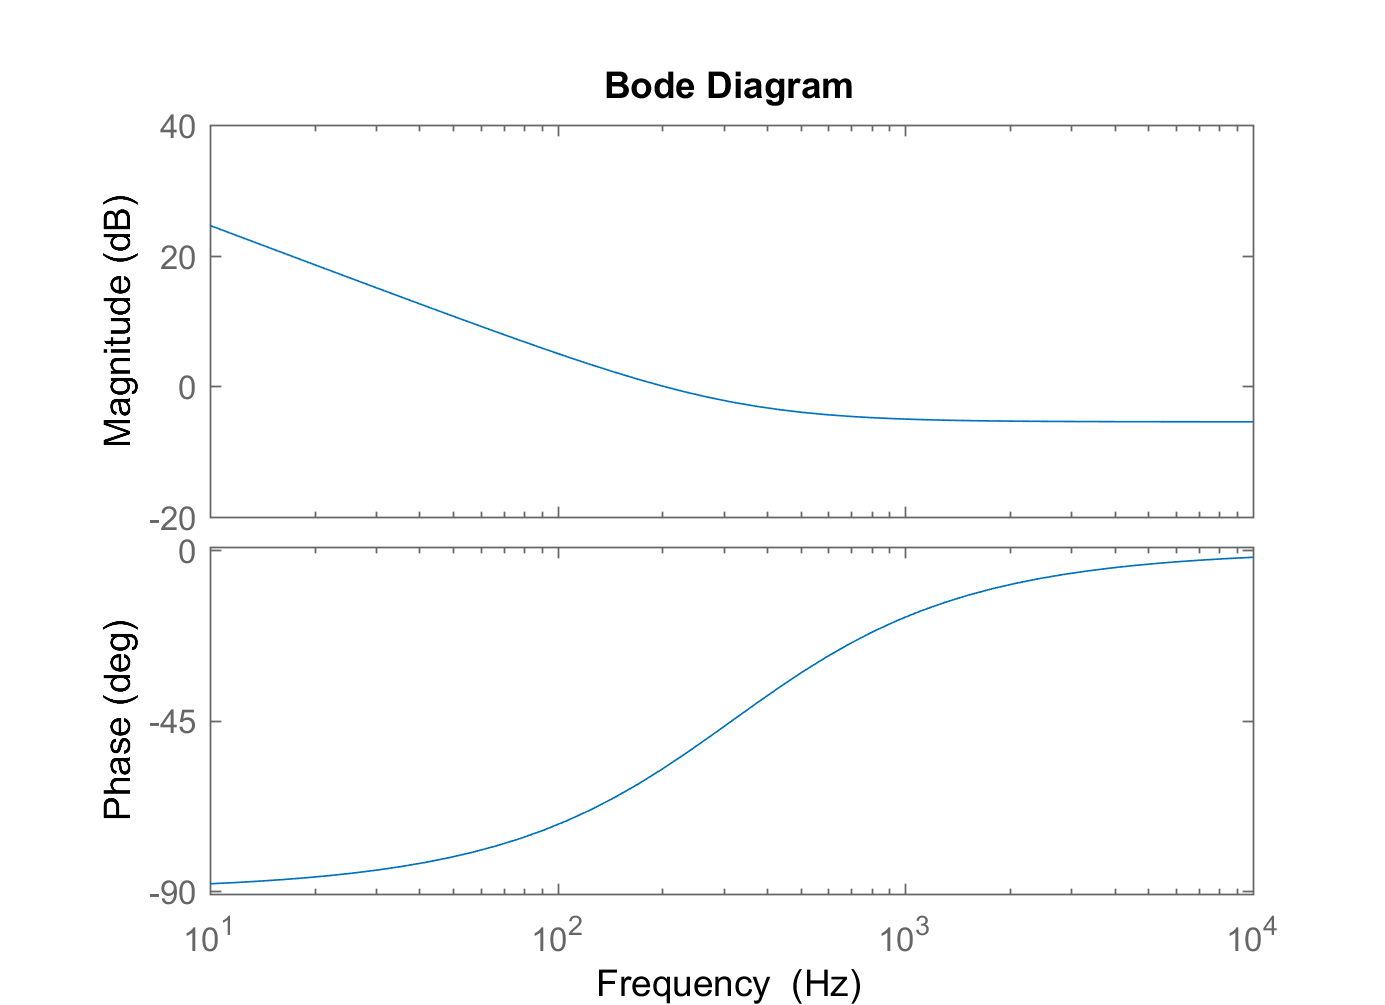
\includegraphics[max width=0.7\linewidth]{/tex/3iteration/billeder/Analyse/MATLAB_error_op_amp.PNG}
	\caption{Bode plot for fejlforstærker}
	\label{fig:MATLAB_error_op_amp_3}
\end{figure}

\noindent Den nye overføringsfunktion for fejlforstærkeren, ganges sammen med overføringsfunktionen for power modulet. Figur~\ref{fig:MATLAB_total_3} viser et bode plot af det samlede system. Det aflæses at converteren vil få en gain-margin på de forventede $10\decibel$, en fasemargin på $72.7^\circ$, og en båndbredde på ca. $3.94k\hertz$. Derudover kan det konstateres at nulpunktet er blevet placeret efter hensigten, da fasen ligger forholdsvis konstant ved frekvenser under $1k\hertz$. 

\begin{figure}[H]
	\center
	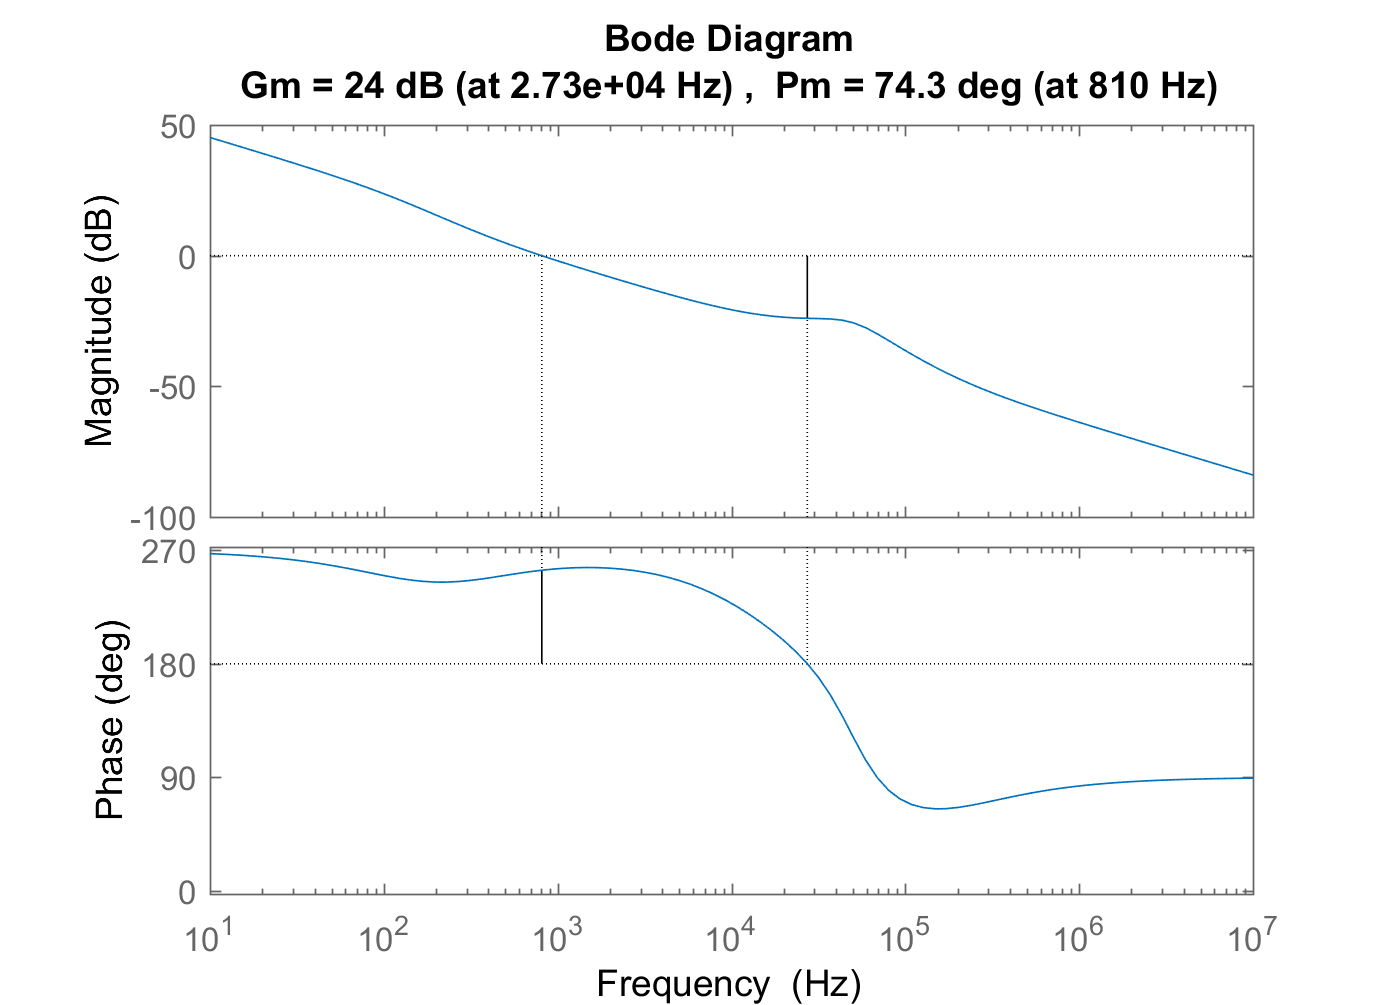
\includegraphics[max width=0.7\linewidth]{/tex/3iteration/billeder/Analyse/MATLAB_total.PNG}
	\caption{Bode plot for det samlede system}
	\label{fig:MATLAB_total_3}
\end{figure}






